\section{Infrastructure}\label{sec:infrastructure}

In figure\ref{fig:project-infra}, we describe our infrastructure that can be first deployed on a local kubernetes single node cluster
with independent DataOps and MLOps pipelines develop by different people with different roles.

by using airflow pipelines as general pipelines to trigger our kubeflow pipelines, we can easily gain in maturity towards
more automation by combining the DataOps pipelines and MLOps pipelines together when they are mature enough.

This way we enable kubeflow features for our model developers within a more general purpose environment.

By using the recent git/sync capabilities of Airflow we can synchronise our dags directly with airflow and
even trigger them automatically in a later stage towards automation.

\begin{figure}[!htbp]
    \centering
    \caption{Proposed MLOps kubernetes infrastructure using GitOps principles}
    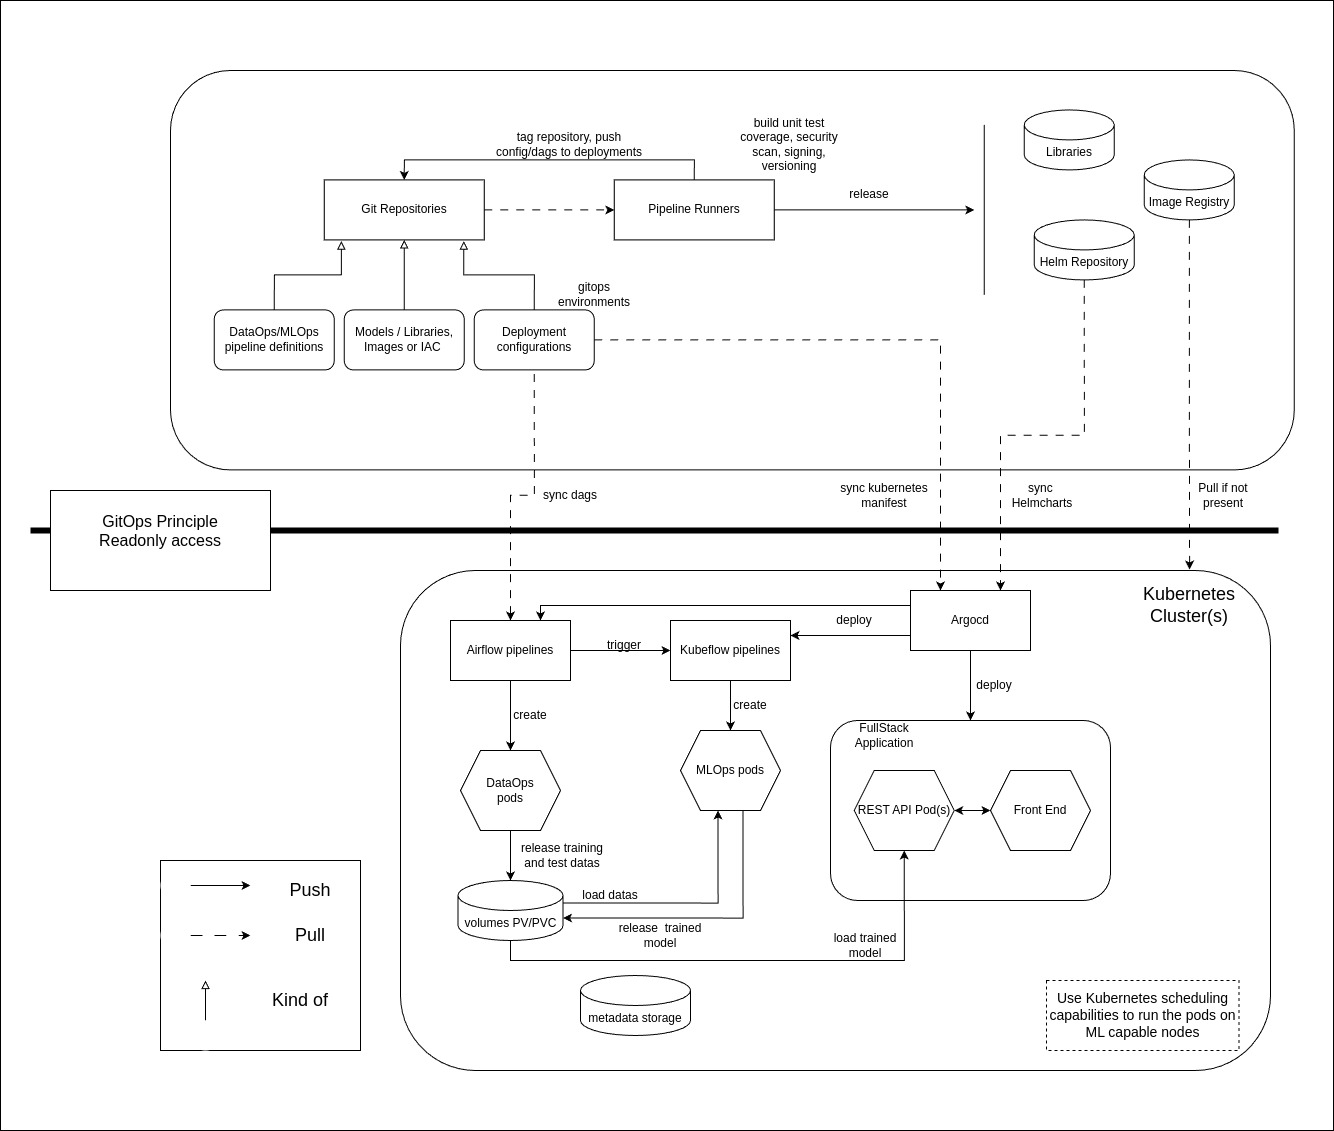
\includegraphics[scale=0.35]{images/project/mthmlops-infra}
    \label{fig:project-infra}
\end{figure}


\subsection{Git Repositories}\label{subsec:git-repositories}
We use Git Repositories for version control and triggering workflow pipeline runners.
We consider 4 types of repositories:

\begin{itemize}
    \item Code Repositories that holds code for models, libraries, docker images and infrastructure as code using Helm.
    \item MLOps and DataOps Pipelines Repositories.
    In our infrastructure those repositories holds the definition of our Airflow DAGs.
    In the first iteration those repositories can also hold images for
    \item Deployment/Configuration repositories.
    Those repositories are used to hold configuration for the deployed applications and Airflow dags.
    We use ArgoCD GitOps implementation to synchronise changes to those repositories.
    Airflow git/sync feature allows us to synchronise our dags with
    Change in those repositories can be automated by the pipeline runners.
    Depending on your team and organization those repositories can be separated into multiple repositories (per team, per domain, per environment (dev,test,staging,prod))
    For the Dev environment we allow developers to push from their code repositories within those repositories.
    For the production environment we use a pipeline to pull the configuration from the staging environment.
    We called this promote our configuration to a new environment.
    In case of full automation the pulling/promotion can be trigger automatically by ArgoCD sending webhooks on any test results desired.
    \item CI/CD pipelines templates
    In those we define workflows that can be used in any repository to be used by the developers.
    It includes building image workflows, versioning with tags on repositories, pushing new configurations into deployments repositories.
    By defining them in a separate repository it allows us to version them and make it easy for developers to choose a workflow.
    Each workflow is closely tight to the structure of the repository, so we defined one per type of repositories.
\end{itemize}

\subsection{GitOps}
With a Helm-based installation pipeline, the runner requires write access to push applications directly to Kubernetes.
By adopting ArgoCD and a GitOps approach, we eliminate this requirement by pulling changes directly from GitHub.
This enables all operations to be managed within GitHub.
However, it necessitates properly configured permissions in GitHub to prevent potential security breaches.

Airflow also integrate a Git/Sync feature that allows us to load and trigger the DAGs within Airflow.

\subsection{DataOps pipelines}
DataOps pipelines are defined as Airflow DAGs that will, with the KubernetesExecutor functionality of Airflow,
create pods for every step defined in the pipeline.
They can be connected to an observability stack like OpenSearch to analyse and store the data.
This can be used as Monitoring tools for all our infrastructure too.

\begin{figure}[!htbp]
    \centering
    \caption{Example of a DataOps pipeline define within Airflow}
    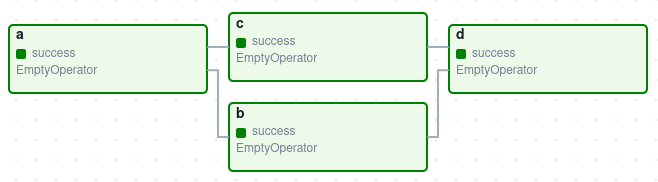
\includegraphics[scale=0.5]{images/project/data-ops-airflow-dag}
    \label{fig:project-data-ops-airflow-dag}
\end{figure}

\subsection{MLOps pipelines}
Kubeflow allows us to deploy all the required steps within our MLOps pipeline by creating pods in the required namespace within our Kubernetes cluster.
A lot like Airflow would.
We use Kubeflow to allow our ML engineer to use other features like model and model metadata storage.

\begin{figure}[!htbp]
    \centering
    \caption{Example of a MLOps pipeline define within Airflow}
    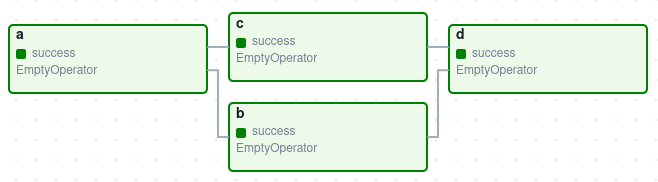
\includegraphics[scale=0.5]{images/project/data-ops-airflow-dag}
    \label{fig:project-ml-ops-airflow-dag}
\end{figure}

